\documentclass[12pt, a4paper]{article}

\usepackage{fullpage}
\usepackage{latexsym}
\usepackage{amsfonts}
\usepackage{amssymb}
\usepackage{graphicx}
\usepackage{amsmath}
\usepackage{float}
\usepackage{subcaption}

\pagestyle{empty}

\begin{document}

\title{{AMATH 568\\
Advanced Differential Equations}\\
{\bf \Huge Homework 8}}

\author{Lucas Cassin Cruz Burke}

\date{Due: March 8, 2023}

\maketitle

\begin{enumerate}
    \item Consider the inverted pendulum dynamics: $$y'' + (\delta + \epsilon \cos \omega t) \sin y = 0$$
    
    \begin{enumerate}
        \item Perform a Floquet analysis (computationally) of the pendulum with continuous forcing $\cos \omega t$. 
        
        \textbf{Solution:} We can use Python's solve-ivp function to directly solve this equation for different values of $\delta$, $\epsilon$, and $\omega$. For each triple $(\delta, \epsilon, \omega)$ we solve the system twice on the interval $t\in [0, \frac{2\pi}{\omega}]$ to find $y_1(t)$ and $y_2(t)$ with initial conditions 

        \begin{align*}
            y_1(0)= y_2'(0)=1 \\ y_2(0)= y_1'(0)=0
        \end{align*}

        We can then use these to define the Floquet discriminant $\Gamma$ as a function of the parameters $\delta$, $\epsilon$, and $\omega$. 
        
        $$\Gamma(\delta, \epsilon, \omega) = y_1(T) + y_2'(T)$$ 

        The stability of the periodic solutions for $(\delta, \epsilon, \omega)$ depends on the condition 

        $$|\Gamma(\delta, \epsilon, \omega)| < 2$$

        Having defined this function in Python, we can directly compute $\Gamma$ for different values of $\delta$, $\epsilon$ and $\omega$ to determine the dependence of the stability on these parameters. 

        \item Evaluate for what values of $\delta$, $\epsilon$, and $\omega$, the pendulum is stabilized. 
        
        \textbf{Solution:} Using the function defined in (a) for numerically computing the Floquet discriminant we can explore the parameter space and see how stability is impacted by $\epsilon, \delta$, and $\omega$. 

        Figures 1, 2 and 3 show the dependence of the Floquet analysis on the underlying parameters. Figure 1 shows the real value of the $\Gamma$, Figure 2 shows the absolute value $|\Gamma|$ For small values of $\omega$, and Figure 3 shows which values satisfy the stability condition $|\Gamma|>2$. 
        
        We observe from these pictures the existence of three behavioral regimes depending on the relative size of $\omega$ to $\delta$ and $\epsilon$.. For small values of $\omega \ll \delta, \epsilon$ we observe the clearest shift in stabilization behavior depending on the relative magnitudes of $\epsilon$ and $\delta$. For $\delta>\epsilon$ we observe a quasi-periodic structure in the Floquet discriminant $\Gamma$ and the pendulum is stabilized for most parameter values. Conversely, for $\epsilon > \delta$ the stabilization structure appears chaotic for $\omega \ll 1$, or at least, the structure cannot be resolved efficiently using this method. However as $\omega$ grows to $\omega \sim \delta, \epsilon$ we observe new phenomena in the $\epsilon > \delta$ region including pattern formation (see $\omega=0.02$) and eventual coherence (see $\omega=0.2$) into a near-uniformly divergent solution. 

        Our observations in the $\omega \gg \delta, \epsilon$ regime agree with the analytical results which predict the pendulum stabilizing for $\omega \rightarrow \infty$. Indeed, we see that $\Gamma \rightarrow 2$ for all $\epsilon, \delta$, implying neutral stability. 

        \begin{figure}[H]
            \centering
            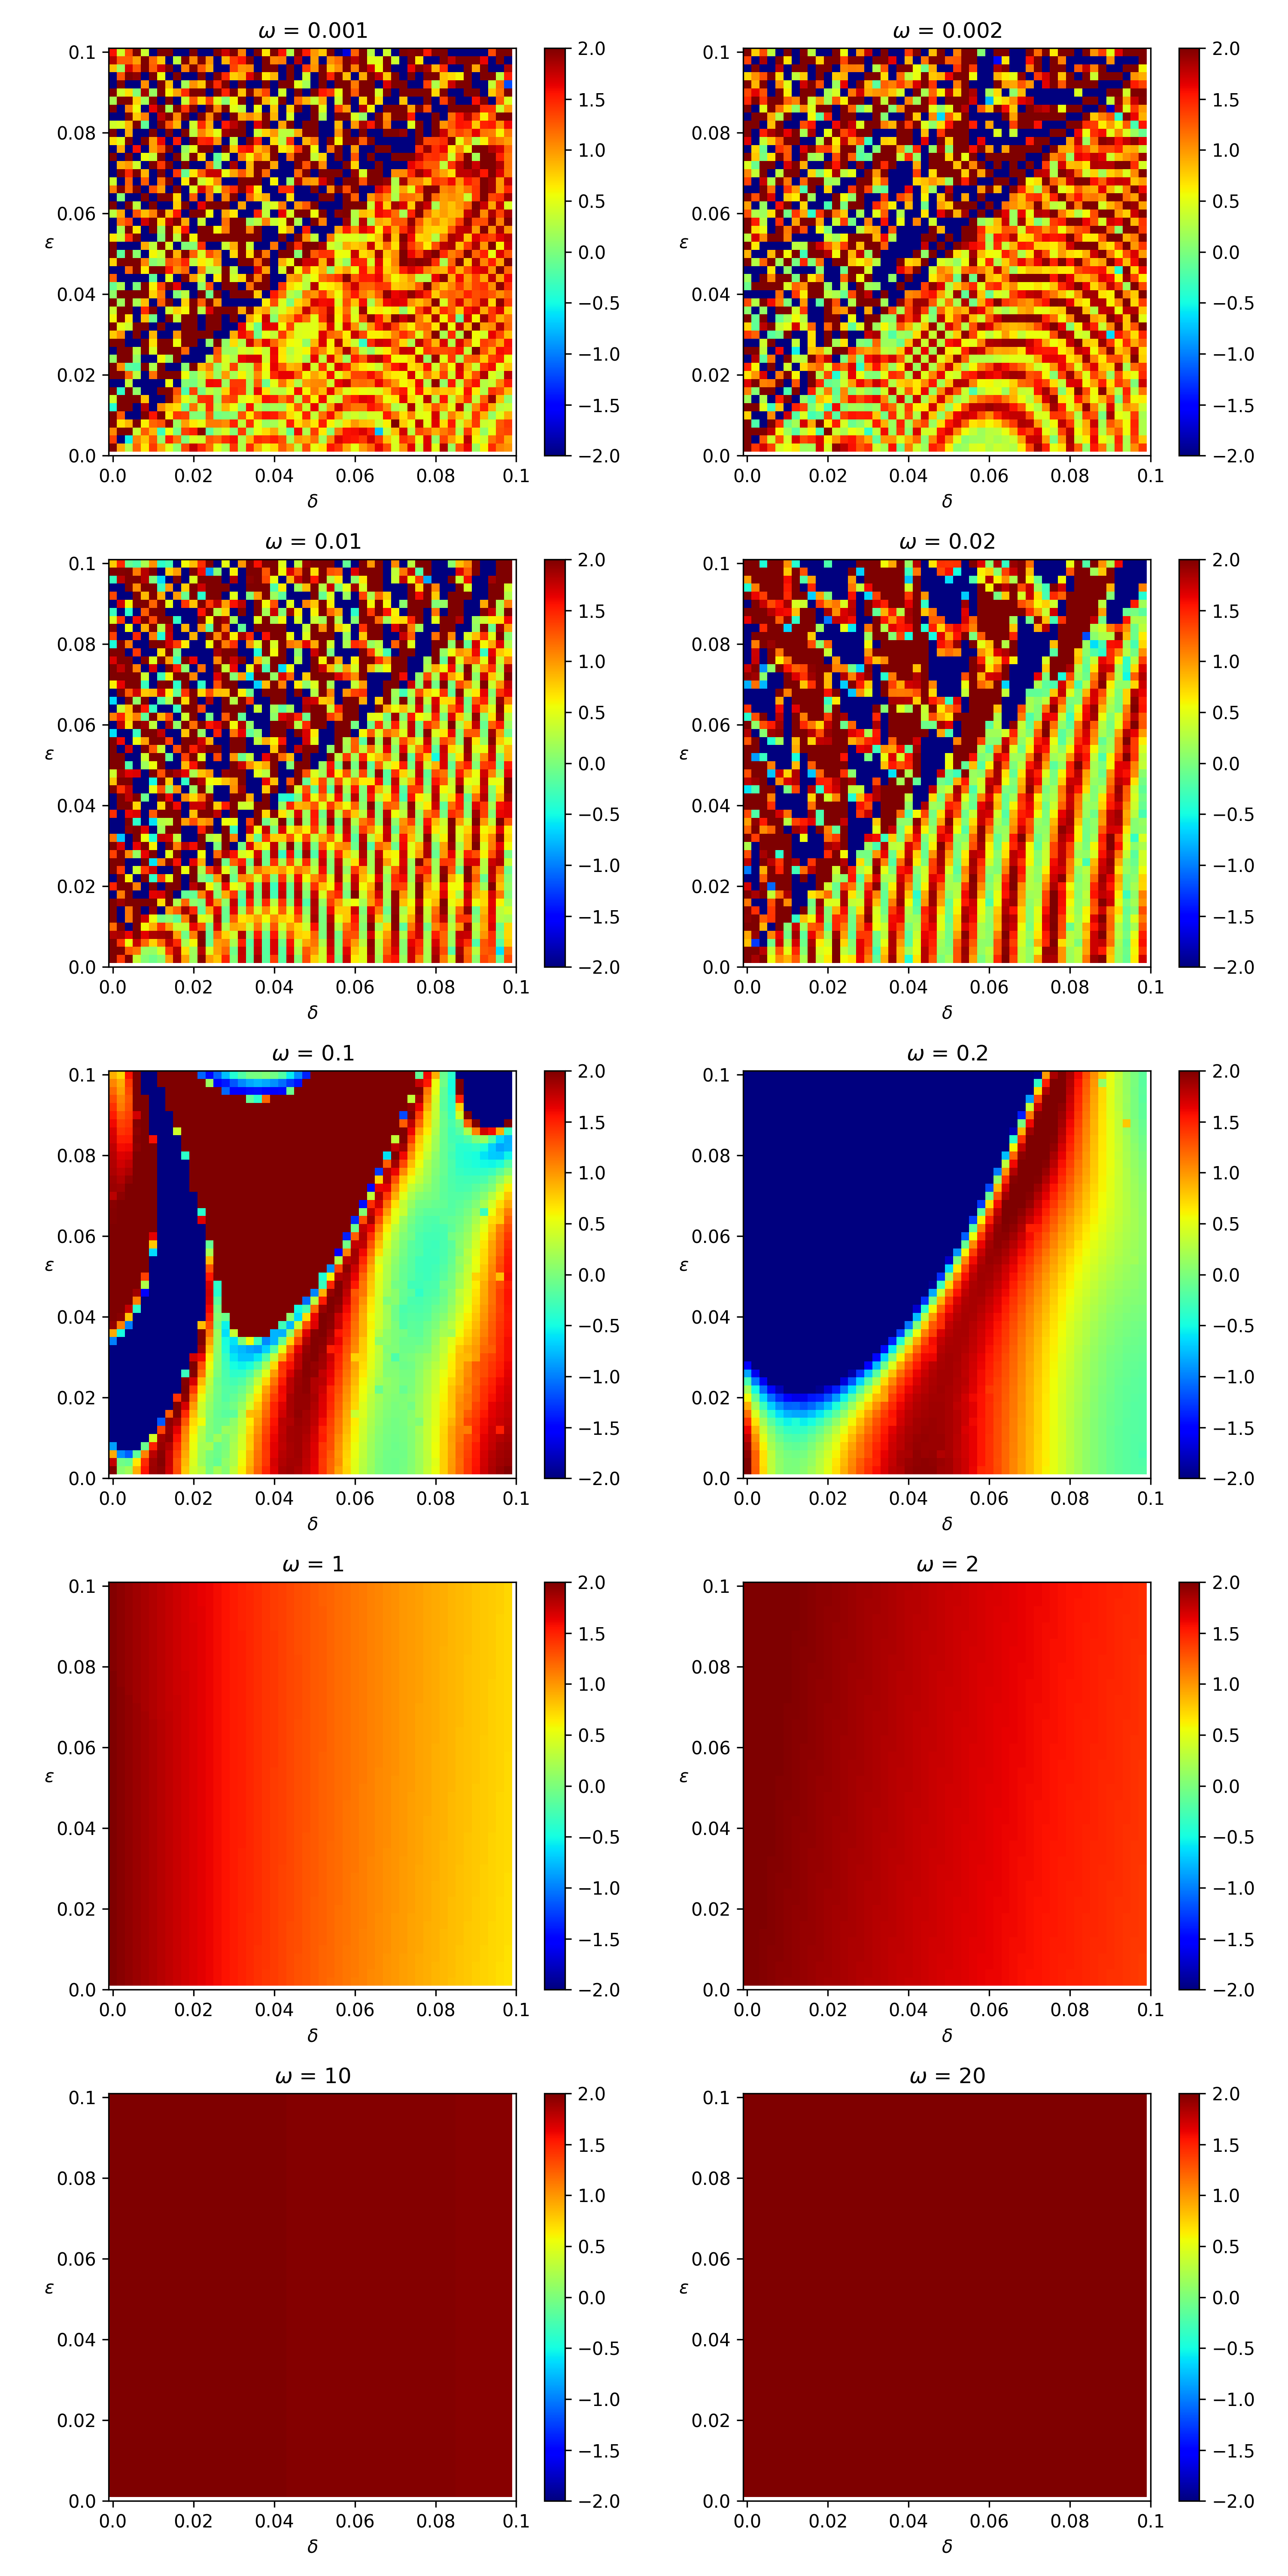
\includegraphics[width=12cm]{Gamma_multi.png}
            \caption{Value of Floquet discriminant $|\Gamma(\delta, \epsilon, \omega)|$ for various parameter values.}
        \end{figure}

        \begin{figure}[H]
            \centering
            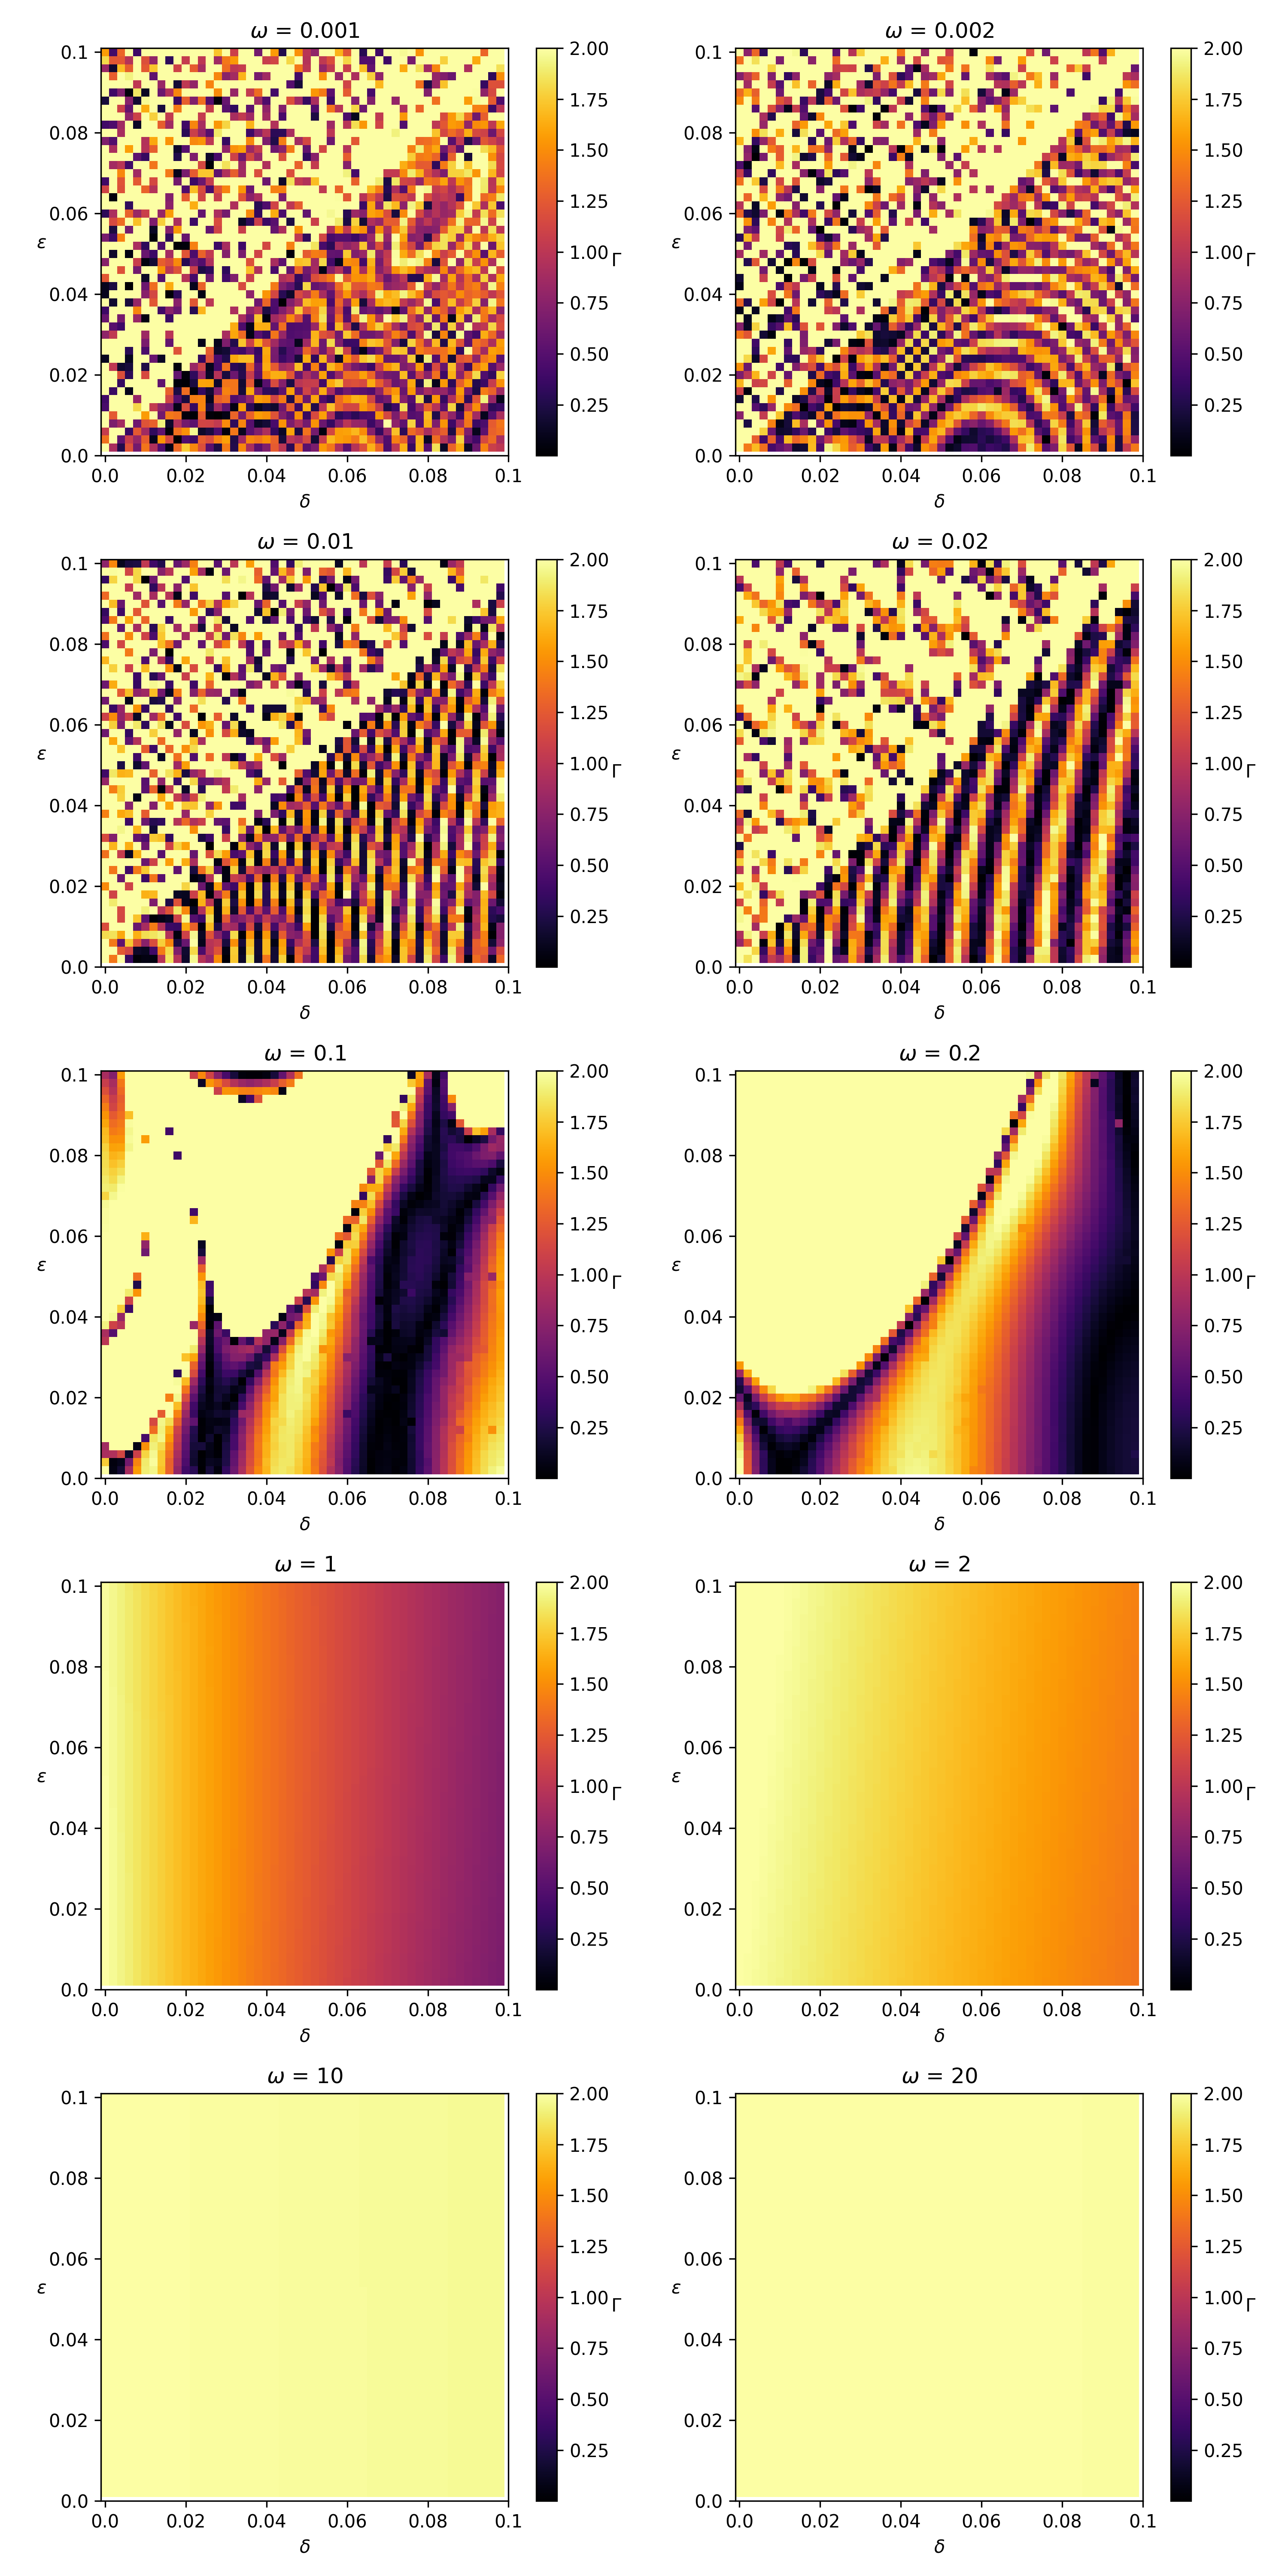
\includegraphics[width=12cm]{Gamma_color.png}
            \caption{Absolute value of Floquet discriminant $|\Gamma(\delta, \epsilon, \omega)|$ for various parameter values.}
        \end{figure}

        \begin{figure}[H]
            \centering
            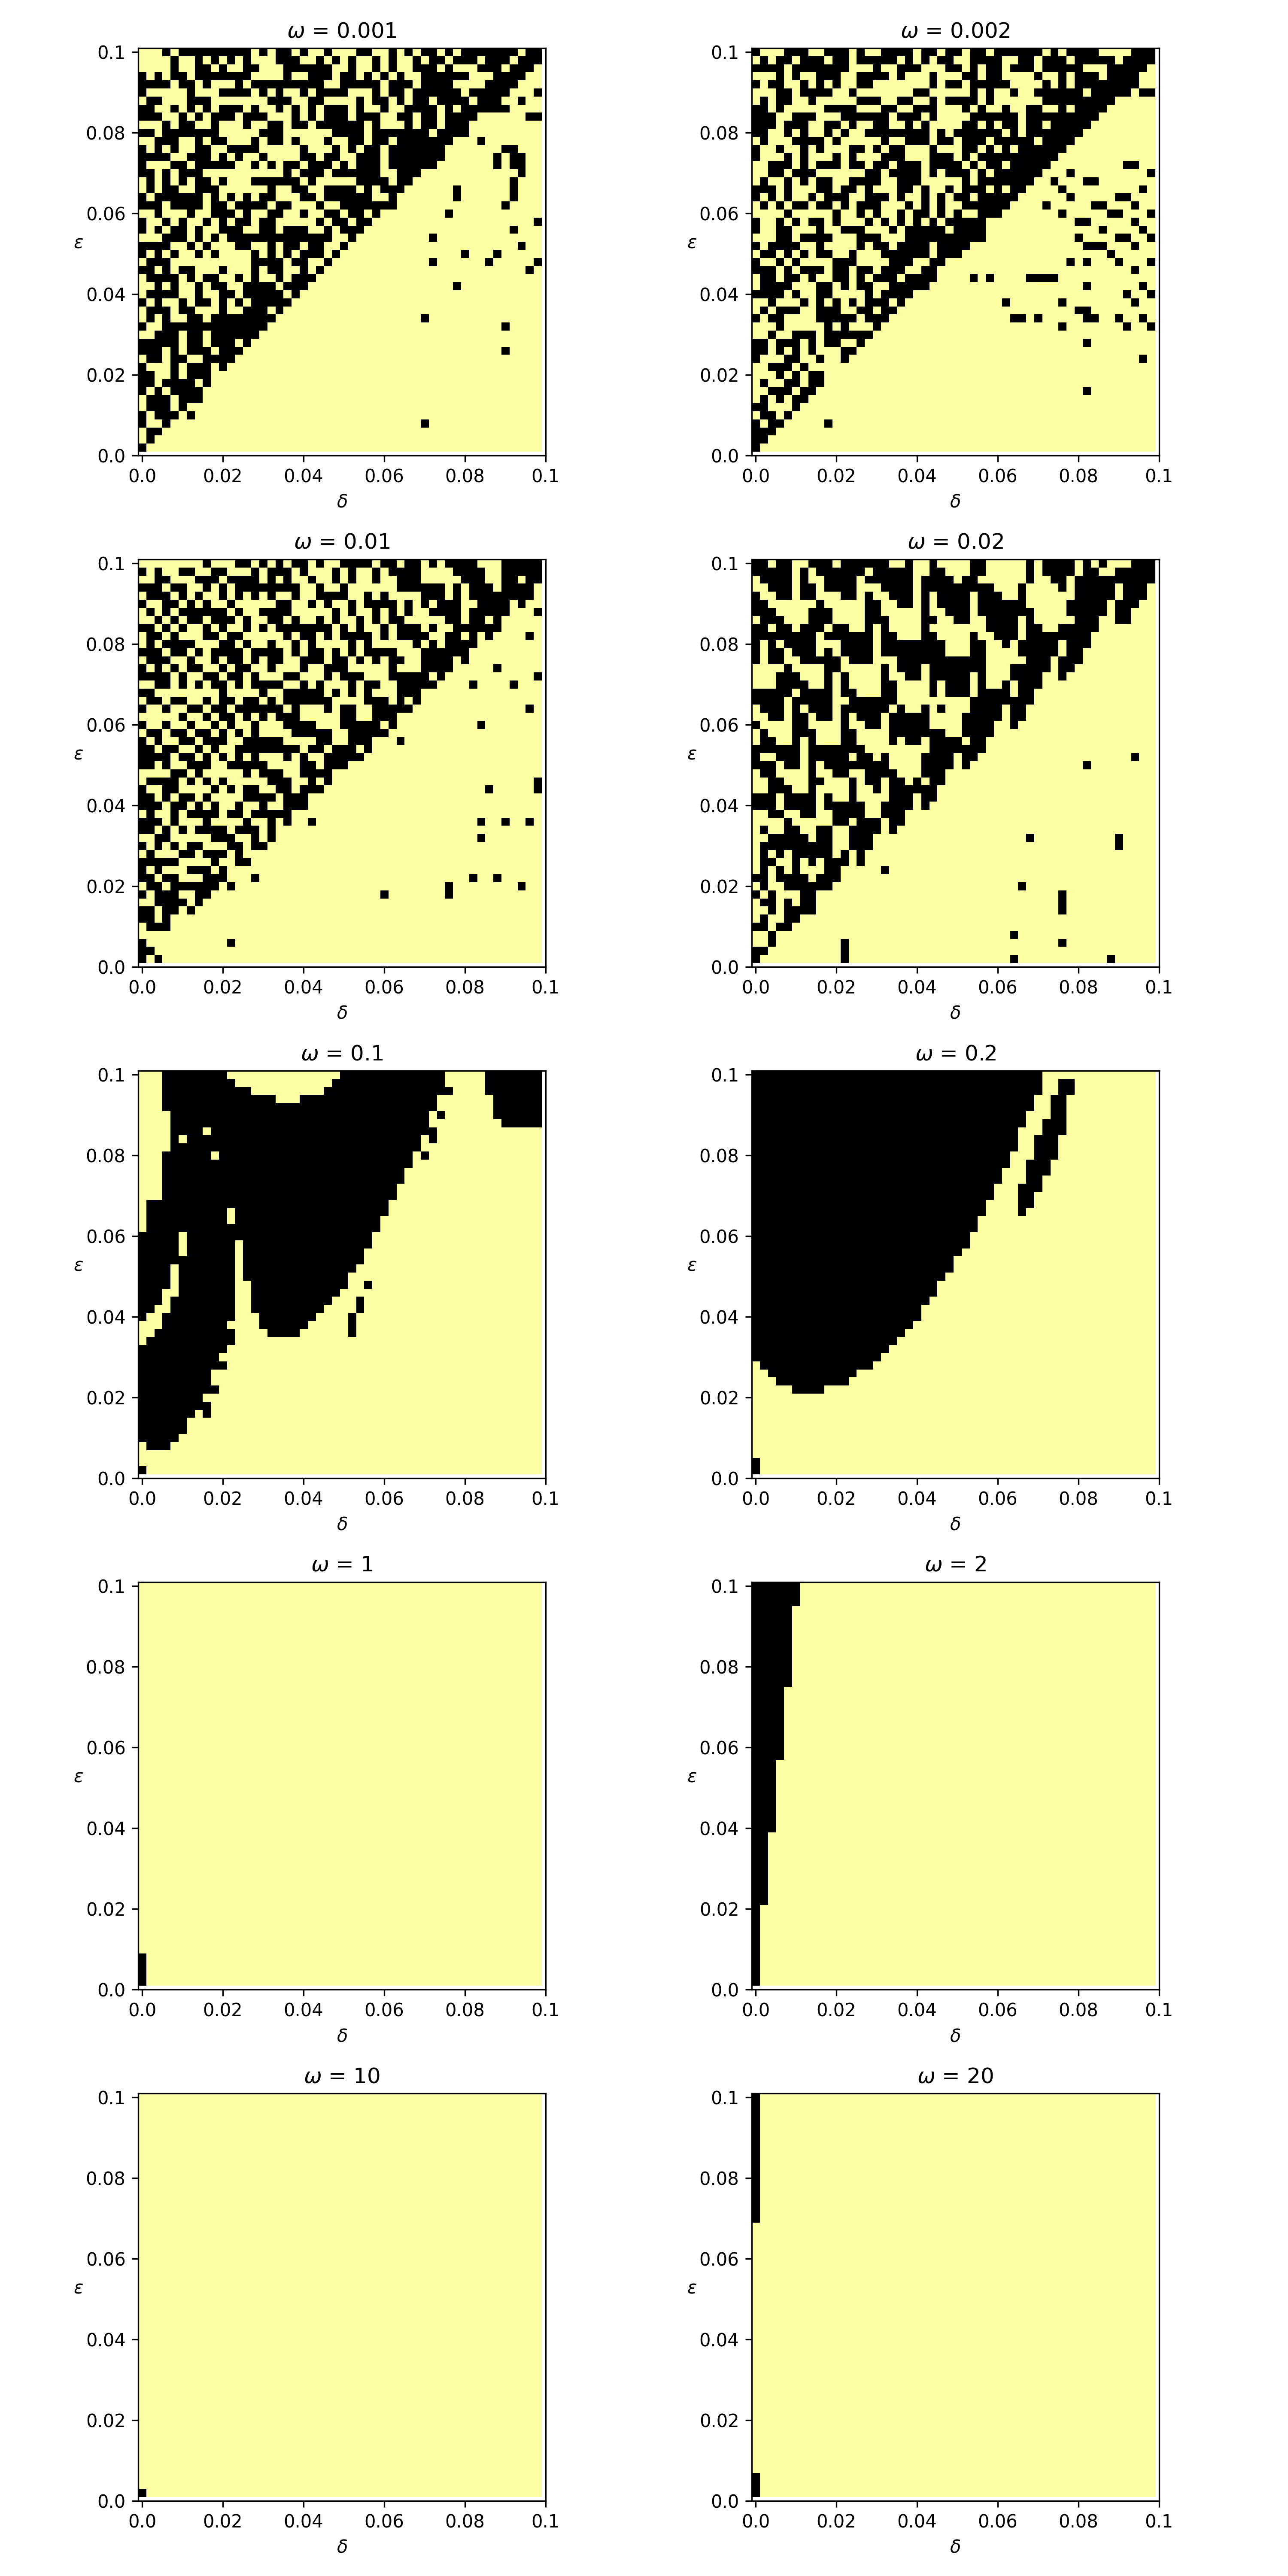
\includegraphics[width=12cm]{Gamma_BW.png}
            \caption{Stability of periodic solutions for parameters $(\delta, \epsilon, \omega)$. Yellow pixels correspond to stabilized pendulum.}
        \end{figure}

        
    \end{enumerate}
\end{enumerate}

\end{document}